\chapter{Experiments}
\label{chap:experiments}
\section{Environment}
We developed our experiments environment cluster were listed as table \ref{talbe:Host}, and created 4 virtual machines in the computer that each of their resource were listed as table \ref{talbe:Virtual Machine}. We mount NFS to each virtual machines, and test 2 type of NFS, hard disk, and memory(tmpfs). In addition, we test difference about dumping new checkpoint image each time and pre-dumping checkpoint image than dumping checkpoint follow pre-dump checkpoint image.

\begin{table}[h]
\begin{center}
\begin{tabular}{|c|c|} \hline
CPU & Intel Xeon(R) CPU-E5-2630 v3 @ 2.40GHx x 32 \\ \hline
Memory & 64 GB \\ \hline
Disk & 1.0T \\ \hline
OS & Ubuntu 15.10 64 bit \\ \hline
Kernel version & 4.4.4-040404-generic \\ \hline
Docker version & 1.10.3 \\ \hline
Docker Swarm version & 1.2 \\ \hline
Virtual Box version & 5.10.14 \\ \hline
\end{tabular}
\end{center}
\caption{Experiment environment}
\label{talbe:Host}
\end{table}

\begin{table}[h]
\begin{center}
\begin{tabular}{|c|c|} \hline
CPU & Intel Xeon(R) CPU-E5-2630 v3 @ 2.40GHx x 4 \\ \hline
Memory & 8 GB \\ \hline
Disk & 40G \\ \hline
OS & Ubuntu 15.10 64 bit \\ \hline
Kernel version & 4.4.4-040404-generic \\ \hline
Docker version & 1.10.3 \\ \hline
Docker Swarm version & 1.2 \\ \hline
\end{tabular}
\end{center}
\caption{Virtual Machine experiment environment}
\label{talbe:Virtual Machine}
\end{table}

\section{Container Migration Time}
As shown in Figure \ref{fig:Docker Swarm migration with remote storage server}, native is a reference line of the other kinds of experiment. We choose redis\cite{paksula2010persisting} as our migration container, because it uses memory to save its data. Therefore, we can check the correctness of redis data to make sure container migration is success.

The first step of Creating the container on another Swarm Node is fast for all environments, because we assume that they already have downloaded their container images from the remote repository, thus, they don't need to transport container images from the other Swarm Node.

Second, if checkpoint ticker has version control of checkpoint the container, the container has to pre-dump the checkpoint image. After pre-dumping the checkpoint image, dump checkpoint will track memory different with the pre-dump checkpoint image. On the other hand, checkpoint ticker dump the checkpoint image directly. The result of total checkpoint time, the version which has pre-dumping one's time is longer then the other one, because it has to add pre-dumping checkpoint time and dumping checkpoint time. Although the version which has pre-dumping one's is longer, but it provides the less frozen time to the container that improves CPU's utilization.

The third step is restoring the container to the container which has already been created in the Swarm Node. except NFS with memory, they all have nearly performance.

The last step, it has big disparity of the delete checkpoint image step at pre-dumping version, because it has more image files and directories than the version without pre-dumping version.

After all, the checkpoint and restoration of container in memory is more faster then hard disk in NFS. As result of Figure \ref{fig:Docker Swarm migration with remote storage server}, NFS with memory has the best performance in this experiment.

\begin{figure}[h]
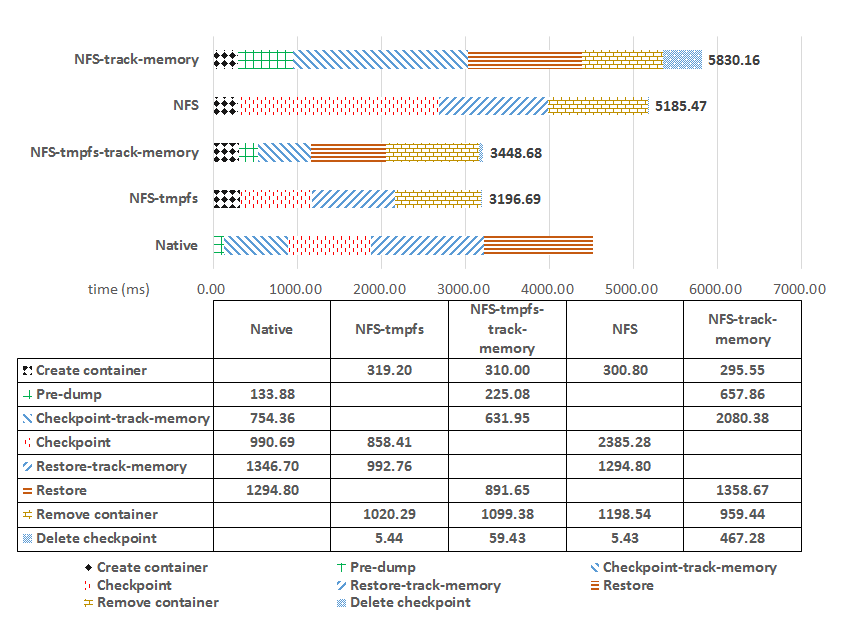
\includegraphics[width=17cm]{figure/migration_time.png}
\caption{Docker Swarm migration with remote storage server}
\label{fig:Docker Swarm migration with remote storage server}
\end{figure}

\section{Container Checkpoint Time Influence of Container Process Time}

\begin{table}[h]
\begin{center}
\begin{tabular}{|c|c|c|c|c|c|} \hline
& Native & NFS-tmpfs & NFS & NFS-tmpfs-version & NFS-version \\ \hline
process time & 30.36 & 31.846 & 35.476 & 31.957 & 35.843 \\ \hline
\end{tabular}
\end{center}
\caption{Container Checkpoint Time of CPU Process}
\label{talbe:Checkpoint Time of CPU}
\end{table}

%\begin{table}[h]
%\begin{center}
%\begin{tabular}{|c|c|c|c|c|} \hline
%& NFS-tmpfs & NFS & NFS-tmpfs-version & NFS-version \\ \hline
%pre-dump & 107.718 & 350.334 & &\\ \hline
%checkpoint-version & 512.071 & 1942.994 & & \\ \hline
%checkpoint & & & 627.706 & 2021.346 \\ \hline
%total & 619.789 & 2293.324 & 627.706 & 2021.346 \\ \hline
%\end{tabular}
%time(ms)
%\end{center}
%\caption{Container Checkpoint Time Influence of Container Process Time}
%\label{talbe:Checkpoint Time Influence CPU}
%\end{table}

\begin{figure}[h]
\begin{center}
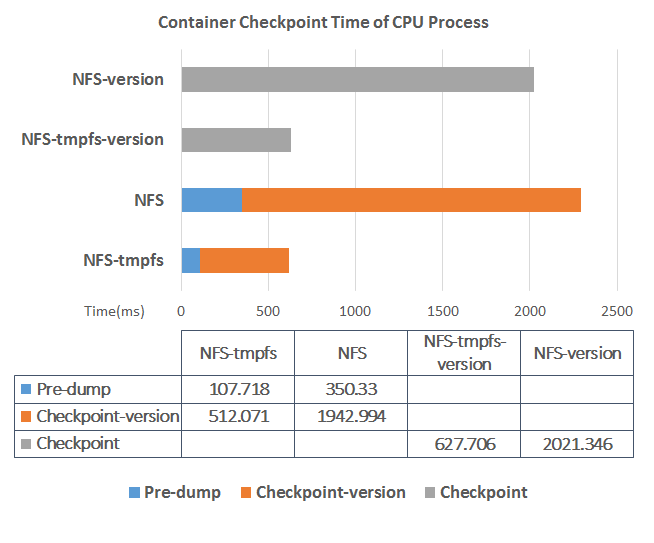
\includegraphics[width=14cm]{figure/cpu_checkpoint_time.png}
\end{center}
\caption{Container Checkpoint Time Influence of Container Process Time}
\label{fig:Checkpoint Time Influence CPU}
\end{figure}